\documentclass[aspectratio=169]{beamer}

% Theme
\usetheme{default}
\usecolortheme{beaver}

% Packages
\usepackage{amsmath,amssymb,amsthm}
\usepackage{mathtools}
\usepackage{bm}
\usepackage{tikz}
\usetikzlibrary{arrows.meta,positioning,calc,patterns,decorations.markings}

% Custom commands
\newcommand{\R}{\mathbb{R}}
\newcommand{\Pp}{\mathcal{P}}
\newcommand{\Mm}{\mathcal{M}}
\newcommand{\Ld}{\mathcal{L}^d}
\newcommand{\Cb}{C_b}
\newcommand{\Czero}{C_0}

% Title
\title{Duality in Optimal Transport}
\subtitle{Chapter 1.2: The Dual Problem}
\author{}
\date{}

\begin{document}

%==============================================================================
\begin{frame}
\titlepage
\end{frame}

%==============================================================================
\begin{frame}[shrink=10]{Outline}
\tableofcontents[hideallsubsections]
\end{frame}

%==============================================================================
\section{Why Duality?}
%==============================================================================

\begin{frame}{Recap: The Kantorovich Problem}
\textbf{Kantorovich Problem (KP):}
\[
\boxed{\textbf{(KP)} \quad \min_{\gamma \in \Pi(\mu,\nu)} \int_{X \times Y} c(x,y) \, d\gamma(x,y)}
\]

\vspace{0.2cm}
\textbf{Key observation:} (KP) is a \textbf{linear optimization} problem!
\begin{itemize}
    \item Objective: $\int c \, d\gamma$ is \textbf{linear} in $\gamma$
    \item Constraints: marginal conditions are \textbf{linear} in $\gamma$
\end{itemize}

\vspace{0.2cm}
\begin{center}
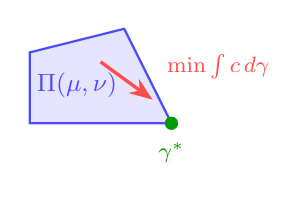
\begin{tikzpicture}[scale=0.6]
    % Feasible region
    \draw[blue!70, thick, fill=blue!10] (0,0) -- (3,0) -- (2,2) -- (0,1.5) -- cycle;
    \node[blue!70, font=\small] at (1, 0.8) {$\Pi(\mu,\nu)$};

    % Objective direction
    \draw[-{Stealth}, red!70, very thick] (1.5, 1.3) -- (2.6, 0.5);
    \node[red!70, font=\footnotesize, right] at (2.7, 1.2) {$\min \int c \, d\gamma$};

    % Optimal point
    \fill[green!60!black] (3, 0) circle (4pt);
    \node[green!60!black, below, font=\footnotesize] at (3, -0.2) {$\gamma^*$};
\end{tikzpicture}
\end{center}
\vspace{-0.3cm}
\begin{center}
\small Linear Program structure
\end{center}
\end{frame}

%==============================================================================
\begin{frame}{Why Study Duality?}
\textbf{Duality theory} for (KP) provides:

\vspace{0.3cm}
\begin{enumerate}
    \item \textbf{Lower bounds} on the optimal transport cost
    \[
    \text{(any dual feasible)} \leq \min(\text{KP})
    \]

    \vspace{0.2cm}
    \item \textbf{Optimality conditions} (complementary slackness)
    \[
    \gamma^* \text{ optimal} \;\Leftrightarrow\; \text{certain conditions on } (\gamma^*, \phi^*, \psi^*)
    \]

    \vspace{0.2cm}
    \item \textbf{Alternative formulation} (often easier to solve)

    \vspace{0.2cm}
    \item \textbf{Economic interpretation} (prices, no-arbitrage)

    \vspace{0.2cm}
    \item \textbf{Characterization of optimal transport maps}
\end{enumerate}

\vspace{0.4cm}
\textbf{Goal:} Find a \textbf{dual problem (DP)} for (KP).
\end{frame}

%==============================================================================
\section{Deriving the Dual Problem}
%==============================================================================

\begin{frame}{Encoding Constraints via Supremum}
\textbf{Key idea:} Express the constraint $\gamma \in \Pi(\mu,\nu)$ as a supremum.

\vspace{0.3cm}
For $\gamma \in \Mm_+(X \times Y)$, consider:
\[
\sup_{\phi, \psi} \left[ \int_X \phi \, d\mu + \int_Y \psi \, d\nu - \int_{X \times Y} (\phi(x) + \psi(y)) \, d\gamma \right]
\]

\vspace{0.2cm}
\textbf{Claim:} This supremum equals:
\[
= \begin{cases}
0 & \text{if } \gamma \in \Pi(\mu,\nu) \\
+\infty & \text{otherwise}
\end{cases}
\]

\vspace{0.3cm}
\textbf{Why?}
\begin{itemize}
    \item If $\gamma \in \Pi(\mu,\nu)$: $\int \phi \, d\mu + \int \psi \, d\nu = \int (\phi(x) + \psi(y)) \, d\gamma$ \quad $\Rightarrow 0$
    \item If $\gamma \notin \Pi(\mu,\nu)$: can find $\phi$ or $\psi$ making the difference arbitrarily large
\end{itemize}
\end{frame}

%==============================================================================
\begin{frame}{The Inf-Sup Formulation}
\textbf{Adding the constraint-encoding term:}
\[
\min_\gamma \int_{X \times Y} c \, d\gamma + \sup_{\phi,\psi} \left[ \int_X \phi \, d\mu + \int_Y \psi \, d\nu - \int_{X \times Y} (\phi(x) + \psi(y)) \, d\gamma \right]
\]

\vspace{0.3cm}
This equals the original (KP): if $\gamma \in \Pi(\mu,\nu)$, the sup term is 0; otherwise $+\infty$.

\vspace{0.4cm}
\textbf{Interchanging inf and sup:}
\[
\boxed{\sup_{\phi,\psi} \left[ \int_X \phi \, d\mu + \int_Y \psi \, d\nu + \underbrace{\inf_{\gamma \geq 0} \int_{X \times Y} (c(x,y) - \phi(x) - \psi(y)) \, d\gamma}_{\text{inner minimization}} \right]}
\]

\vspace{0.3cm}
\textbf{Question:} When is $\min \sup = \sup \min$? (Minimax theorems)
\end{frame}

%==============================================================================
\begin{frame}{Computing the Inner Infimum}
\textbf{Inner problem:}
\[
\inf_{\gamma \geq 0} \int_{X \times Y} \underbrace{(c(x,y) - \phi(x) - \psi(y))}_{\text{integrand}} \, d\gamma
\]

\vspace{0.3cm}
\textbf{Analysis:}
\begin{itemize}
    \item If $\phi(x) + \psi(y) > c(x,y)$ for some $(x,y)$:
    \begin{itemize}
        \item Concentrate mass on that point with mass $\to \infty$
        \item Integral $\to -\infty$
    \end{itemize}
    \item If $\phi(x) + \psi(y) \leq c(x,y)$ for all $(x,y)$:
    \begin{itemize}
        \item Integrand $\geq 0$ everywhere
        \item Minimum achieved at $\gamma = 0$, giving value $0$
    \end{itemize}
\end{itemize}

\vspace{0.3cm}
\textbf{Result:}
\[
\inf_{\gamma \geq 0} \int (c - \phi \oplus \psi) \, d\gamma =
\begin{cases}
0 & \text{if } \phi \oplus \psi \leq c \text{ on } X \times Y \\
-\infty & \text{otherwise}
\end{cases}
\]

where $(\phi \oplus \psi)(x,y) := \phi(x) + \psi(y)$.
\end{frame}

%==============================================================================
\begin{frame}{The Dual Problem (DP)}
\begin{block}{Problem 1.9: Dual Problem}
Given $\mu \in \Pp(X)$, $\nu \in \Pp(Y)$, and cost $c: X \times Y \to [0, +\infty]$:
\[
\boxed{\textbf{(DP)} \quad \max \left\{ \int_X \underbrace{\phi \, d\mu}_{\text{payment at source}} + \int_Y \underbrace{\psi \, d\nu}_{\text{receipt at target}} \;:\; \underbrace{\phi \oplus \psi \leq c}_{\text{no arbitrage}} \right\}}
\]
\end{block}

\vspace{0.3cm}
\begin{center}
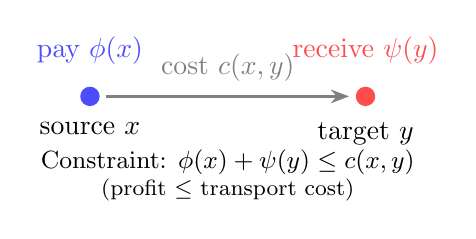
\begin{tikzpicture}[scale=0.7]
    % Source
    \fill[blue!70] (0, 0) circle (5pt);
    \node[below] at (0, -0.3) {source $x$};
    \node[above, blue!70] at (0, 0.4) {pay $\phi(x)$};

    % Target
    \fill[red!70] (5, 0) circle (5pt);
    \node[below] at (5, -0.3) {target $y$};
    \node[above, red!70] at (5, 0.4) {receive $\psi(y)$};

    % Transport
    \draw[-{Stealth}, thick, gray] (0.3, 0) -- (4.7, 0);
    \node[above, gray] at (2.5, 0.1) {cost $c(x,y)$};

    % Constraint
    \node at (2.5, -1.2) {\small Constraint: $\phi(x) + \psi(y) \leq c(x,y)$};
    \node[font=\footnotesize] at (2.5, -1.7) {(profit $\leq$ transport cost)};
\end{tikzpicture}
\end{center}
\end{frame}

%==============================================================================
\begin{frame}{Economic Interpretation}
\begin{columns}
\begin{column}{0.53\textwidth}
\textbf{Shipping company perspective:}
\begin{itemize}
    \item $\phi(x)$: price paid to \textbf{pick up} goods at $x$
    \item $\psi(y)$: price received for \textbf{delivering} goods at $y$
    \item $c(x,y)$: actual cost of transport $x \to y$
\end{itemize}

\vspace{0.2cm}
\textbf{No-arbitrage condition:}
\[
\underbrace{\phi(x) + \psi(y)}_{\text{total revenue}} \leq \underbrace{c(x,y)}_{\text{transport cost}}
\]

Otherwise: infinite profit by arbitrage!

\vspace{0.2cm}
\textbf{Dual objective:} Maximize $\int_X \phi \, d\mu + \int_Y \psi \, d\nu$
\end{column}
\begin{column}{0.47\textwidth}
\begin{center}
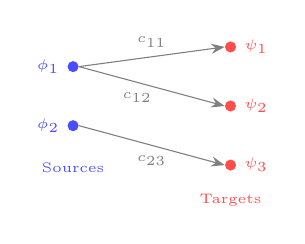
\begin{tikzpicture}[scale=0.5]
    % Sources
    \foreach \y/\p in {2.5/\phi_1, 1/\phi_2} {
        \fill[blue!70] (0, \y) circle (4pt);
        \node[left, blue!70, font=\tiny] at (-0.1, \y) {$\p$};
    }
    \node[below, blue!70, font=\tiny] at (0, 0.3) {Sources};

    % Targets
    \foreach \y/\p in {3/\psi_1, 1.5/\psi_2, 0/\psi_3} {
        \fill[red!70] (4, \y) circle (4pt);
        \node[right, red!70, font=\tiny] at (4.1, \y) {$\p$};
    }
    \node[below, red!70, font=\tiny] at (4, -0.5) {Targets};

    % Some connections with costs
    \draw[gray, -{Stealth}] (0.15, 2.5) -- node[above, font=\tiny] {$c_{11}$} (3.85, 3);
    \draw[gray, -{Stealth}] (0.15, 2.5) -- node[below, font=\tiny, pos=0.4] {$c_{12}$} (3.85, 1.5);
    \draw[gray, -{Stealth}] (0.15, 1) -- node[below, font=\tiny] {$c_{23}$} (3.85, 0);
\end{tikzpicture}
\end{center}
\end{column}
\end{columns}
\end{frame}

%==============================================================================
\section{Weak Duality}
%==============================================================================

\begin{frame}{Weak Duality Theorem}
\begin{block}{Theorem (Weak Duality)}
\vspace{-0.1cm}
\[
\boxed{\sup(\text{DP}) \leq \min(\text{KP})}
\]
\vspace{-0.2cm}
\end{block}

\textbf{Proof:} Take any admissible $(\phi, \psi)$ for (DP) and any $\gamma \in \Pi(\mu,\nu)$.

\vspace{0.1cm}
From constraint $\phi(x) + \psi(y) \leq c(x,y)$, integrate w.r.t. $\gamma$:
\[
\int_{X \times Y} (\phi(x) + \psi(y)) \, d\gamma \leq \int_{X \times Y} c(x,y) \, d\gamma
\]
\vspace{-0.1cm}

Since $\gamma \in \Pi(\mu,\nu)$:
\[
\underbrace{\int_X \phi \, d\mu + \int_Y \psi \, d\nu}_{\text{dual objective}} = \int_{X \times Y} (\phi \oplus \psi) \, d\gamma \leq \int_{X \times Y} c \, d\gamma
\]
\vspace{-0.1cm}

This holds for all admissible $(\phi,\psi)$ and all $\gamma \in \Pi(\mu,\nu)$. \hfill $\square$
\end{frame}

%==============================================================================
\begin{frame}{Weak Duality: Visualization}
\begin{center}
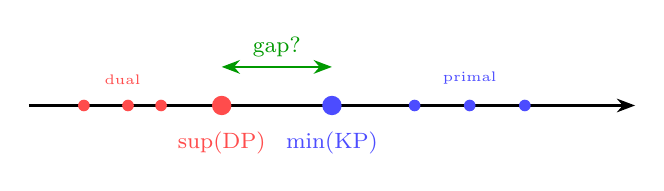
\begin{tikzpicture}[scale=0.7]
    % Number line
    \draw[-{Stealth}, thick] (0,0) -- (11,0);

    % Dual values (lower bounds)
    \fill[red!70] (1, 0) circle (3pt);
    \fill[red!70] (1.8, 0) circle (3pt);
    \fill[red!70] (2.4, 0) circle (3pt);
    \node[red!70, above, font=\tiny] at (1.7, 0.2) {dual};

    % Optimal dual
    \fill[red!70] (3.5, 0) circle (5pt);
    \node[red!70, below, font=\footnotesize] at (3.5, -0.3) {$\sup$(DP)};

    % Gap arrow (positioned higher)
    \draw[{Stealth}-{Stealth}, green!60!black, thick] (3.5, 0.7) -- node[above, font=\footnotesize] {gap?} (5.5, 0.7);

    % Optimal primal
    \fill[blue!70] (5.5, 0) circle (5pt);
    \node[blue!70, below, font=\footnotesize] at (5.5, -0.3) {$\min$(KP)};

    % Primal values (upper bounds)
    \fill[blue!70] (7, 0) circle (3pt);
    \fill[blue!70] (8, 0) circle (3pt);
    \fill[blue!70] (9, 0) circle (3pt);
    \node[blue!70, above, font=\tiny] at (8, 0.2) {primal};
\end{tikzpicture}

\vspace{0.3cm}
\[
\underbrace{\sup(\text{DP})}_{\text{best lower bound}} \leq \underbrace{\min(\text{KP})}_{\text{optimal cost}}
\]
\end{center}

\vspace{0.3cm}
\textbf{Strong Duality:} Under suitable conditions: $\sup(\text{DP}) = \min(\text{KP})$

\vspace{0.1cm}
(No duality gap! Proof in Section 1.6)
\end{frame}

%==============================================================================
\begin{frame}{Exercise 1: Weak Duality Verification}
\textbf{Problem:} Consider $X = Y = \{0, 1\}$ with:
\[
\mu = \frac{1}{2}\delta_0 + \frac{1}{2}\delta_1, \quad \nu = \frac{1}{2}\delta_0 + \frac{1}{2}\delta_1, \quad c(x,y) = |x-y|
\]

\vspace{0.3cm}
\textbf{Questions:}
\begin{enumerate}
    \item[(a)] Write the primal (KP) as a matrix optimization problem.
    \item[(b)] Write all constraints for the dual (DP).
    \item[(c)] Find a feasible dual solution and verify weak duality.
    \item[(d)] Find the optimal solutions and verify strong duality.
\end{enumerate}

\vspace{0.3cm}
\textit{Hint:} The cost matrix is $C = \begin{pmatrix} 0 & 1 \\ 1 & 0 \end{pmatrix}$.
\end{frame}

%==============================================================================
\begin{frame}{Solution 1 (a)-(b)}
\textbf{(a) Primal:} $\min \gamma_{01} + \gamma_{10}$ \quad s.t. row/col sums $= (1/2, 1/2)$

\vspace{0.1cm}
\textbf{(b) Dual constraints:}
\[
\phi_0 + \psi_0 \leq 0, \quad \phi_0 + \psi_1 \leq 1, \quad \phi_1 + \psi_0 \leq 1, \quad \phi_1 + \psi_1 \leq 0
\]
\vspace{-0.3cm}

\begin{center}
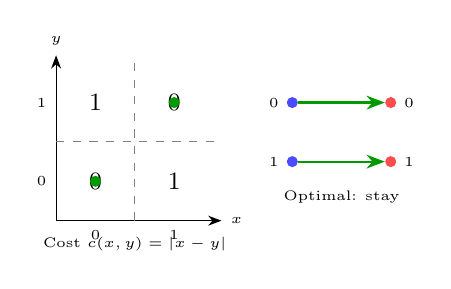
\begin{tikzpicture}[scale=0.5]
    % Cost matrix visualization
    \draw[-{Stealth}] (0,0) -- (4.2,0) node[right, font=\tiny] {$x$};
    \draw[-{Stealth}] (0,0) -- (0,4.2) node[above, font=\tiny] {$y$};
    \draw[gray, dashed] (0,2) -- (4,2);
    \draw[gray, dashed] (2,0) -- (2,4);
    \node[font=\small] at (1, 1) {$0$}; \node[font=\small] at (3, 1) {$1$};
    \node[font=\small] at (1, 3) {$1$}; \node[font=\small] at (3, 3) {$0$};
    \node[below, font=\tiny] at (1, 0) {$0$};
    \node[below, font=\tiny] at (3, 0) {$1$};
    \node[left, font=\tiny] at (0, 1) {$0$};
    \node[left, font=\tiny] at (0, 3) {$1$};
    \fill[green!60!black] (1, 1) circle (4pt);
    \fill[green!60!black] (3, 3) circle (4pt);
    \node[font=\tiny] at (2, -0.6) {Cost $c(x,y)=|x-y|$};

    % Transport arrows on the right
    \begin{scope}[xshift=6cm]
    \fill[blue!70] (0, 3) circle (4pt); \node[left, font=\tiny] at (-0.1, 3) {$0$};
    \fill[blue!70] (0, 1.5) circle (4pt); \node[left, font=\tiny] at (-0.1, 1.5) {$1$};
    \fill[red!70] (2.5, 3) circle (4pt); \node[right, font=\tiny] at (2.6, 3) {$0$};
    \fill[red!70] (2.5, 1.5) circle (4pt); \node[right, font=\tiny] at (2.6, 1.5) {$1$};
    \draw[-{Stealth}, green!60!black, thick] (0.15, 3) -- (2.35, 3);
    \draw[-{Stealth}, green!60!black, thick] (0.15, 1.5) -- (2.35, 1.5);
    \node[font=\tiny] at (1.25, 0.6) {Optimal: stay};
    \end{scope}
\end{tikzpicture}
\end{center}
\end{frame}

%==============================================================================
\begin{frame}{Solution 1 (c)-(d)}
\textbf{(c) Feasible dual:} $\phi = (0,0)$, $\psi = (0,0)$

\quad Dual value $= 0$, Primal value $\geq 0$ \checkmark

\vspace{0.3cm}
\textbf{(d) Optimal:}
\[
\gamma^* = \begin{pmatrix} 1/2 & 0 \\ 0 & 1/2 \end{pmatrix}, \quad K(\gamma^*) = 0
\]

$\phi^* = (0,0)$, $\psi^* = (0,0)$, dual value $= 0$

\vspace{0.3cm}
\textbf{Strong duality verification:}
\[
\underbrace{\int \phi^* d\mu + \int \psi^* d\nu}_{= 0} = \underbrace{\int c \, d\gamma^*}_{= 0} \quad \checkmark
\]
\end{frame}

%==============================================================================
\section{Existence of Dual Solutions}
%==============================================================================

\begin{frame}{Box 1.7: Ascoli-Arzel\`a Theorem}
\begin{block}{Theorem (Ascoli-Arzel\`a)}
Let $X$ be a \textbf{compact} metric space and $f_n: X \to \R$ be a sequence of functions.

If $(f_n)$ is:
\begin{enumerate}
    \item \textbf{Equicontinuous:} $\forall \varepsilon > 0$, $\exists \delta > 0$ such that
    \[
    d(x,y) < \delta \;\Rightarrow\; |f_n(x) - f_n(y)| < \varepsilon \quad \forall n
    \]
    \item \textbf{Equibounded:} $\exists C$ such that $|f_n(x)| \leq C$ for all $x \in X$, all $n$
\end{enumerate}

Then $(f_n)$ has a \textbf{uniformly convergent} subsequence $f_{n_k} \to f$.
\end{block}

\vspace{0.2cm}
\textbf{Converse:} A subset of $C(X)$ is relatively compact (for uniform convergence) iff it is equicontinuous and equibounded.
\end{frame}

%==============================================================================
\begin{frame}{Equicontinuity: Visualization}
\begin{columns}
\begin{column}{0.5\textwidth}
\textbf{Equicontinuous family:}

All functions have ``similar'' oscillation
\begin{center}
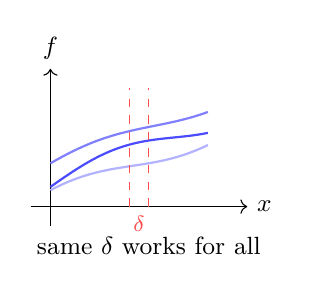
\begin{tikzpicture}[scale=0.5]
    \draw[->] (-0.5,0) -- (5,0) node[right] {\small $x$};
    \draw[->] (0,-0.5) -- (0,3.5) node[above] {\small $f$};

    % Multiple functions with similar slope
    \draw[blue!70, thick] plot[smooth, domain=0:4] (\x, {0.5 + 0.4*\x + 0.3*sin(\x*180/3.14)});
    \draw[blue!50, thick] plot[smooth, domain=0:4] (\x, {1 + 0.4*\x + 0.2*sin(\x*180/3.14 + 30)});
    \draw[blue!30, thick] plot[smooth, domain=0:4] (\x, {0.2 + 0.4*\x + 0.25*sin(\x*180/3.14 + 60)});

    % Delta-epsilon box
    \draw[red!70, dashed] (2, 0) -- (2, 3);
    \draw[red!70, dashed] (2.5, 0) -- (2.5, 3);
    \node[red!70, below, font=\footnotesize] at (2.25, 0) {$\delta$};

    \node at (2.5, -1) {\small same $\delta$ works for all};
\end{tikzpicture}
\end{center}
\end{column}
\begin{column}{0.5\textwidth}
\textbf{NOT equicontinuous:}

Some functions oscillate wildly
\begin{center}
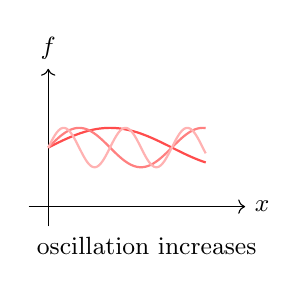
\begin{tikzpicture}[scale=0.5]
    \draw[->] (-0.5,0) -- (5,0) node[right] {\small $x$};
    \draw[->] (0,-0.5) -- (0,3.5) node[above] {\small $f$};

    % Functions with increasing frequency
    \draw[red!70, thick] plot[smooth, domain=0:4, samples=50] (\x, {1.5 + 0.5*sin(\x*180/3.14)});
    \draw[red!50, thick] plot[smooth, domain=0:4, samples=100] (\x, {1.5 + 0.5*sin(\x*360/3.14)});
    \draw[red!30, thick] plot[smooth, domain=0:4, samples=200] (\x, {1.5 + 0.5*sin(\x*720/3.14)});

    \node at (2.5, -1) {\small oscillation increases};
\end{tikzpicture}
\end{center}
\end{column}
\end{columns}

\vspace{0.3cm}
\textbf{Key point:} Equicontinuity provides the compactness needed for existence of dual solutions.
\end{frame}

%==============================================================================
\section{The c-Transform}
%==============================================================================

\begin{frame}{Definition 1.10: c-Transform}
\begin{block}{Definition (c-transform)}
Given $\chi: X \to \R$, the \textbf{c-transform} $\chi^c: Y \to \overline{\R}$ is:
\[
\boxed{\chi^c(y) := \inf_{x \in X} \left[ c(x,y) - \chi(x) \right]}
\]
\end{block}

\begin{block}{Definition ($\bar{c}$-transform)}
Given $\zeta: Y \to \R$, the \textbf{$\bar{c}$-transform} $\zeta^{\bar{c}}: X \to \overline{\R}$ is:
\[
\boxed{\zeta^{\bar{c}}(x) := \inf_{y \in Y} \left[ c(x,y) - \zeta(y) \right]}
\]
\end{block}

\textbf{Terminology:} $\psi$ is \textbf{$\bar{c}$-concave} if $\psi = \chi^c$; \quad $\phi$ is \textbf{c-concave} if $\phi = \zeta^{\bar{c}}$
\end{frame}

%==============================================================================
\begin{frame}{c-Transform: Geometric Interpretation}
\begin{columns}
\begin{column}{0.5\textwidth}
\textbf{For fixed $y$:}
\[
\chi^c(y) = \inf_x \left[ c(x,y) - \chi(x) \right]
\]

\vspace{0.2cm}
\begin{itemize}
    \item View $c(\cdot, y) - \chi(\cdot)$ as a function of $x$
    \item $\chi^c(y)$ is its minimum value
\end{itemize}

\vspace{0.3cm}
\textbf{Analogy with convex conjugate:}

Legendre transform: $f^*(p) = \sup_x [px - f(x)]$

c-transform: $\chi^c(y) = \inf_x [c(x,y) - \chi(x)]$
\end{column}
\begin{column}{0.5\textwidth}
\begin{center}
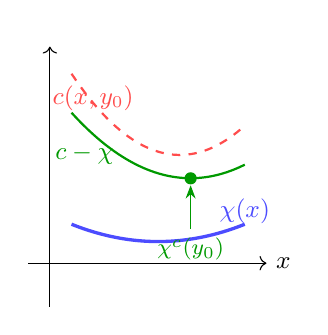
\begin{tikzpicture}[scale=0.55]
    \draw[->] (-0.5,0) -- (5,0) node[right] {\small $x$};
    \draw[->] (0,-1) -- (0,5) node[above] {};

    % chi(x) - coefficient 0.1 so c-chi opens upward
    \draw[blue!70, very thick] plot[smooth, domain=0.5:4.5] (\x, {0.5 + 0.1*(\x-2.5)^2});
    \node[blue!70] at (4.5, 1.2) {\small $\chi(x)$};

    % c(x,y) for fixed y - coefficient 0.3
    \draw[red!70, thick, dashed] plot[smooth, domain=0.5:4.5] (\x, {2.5 + 0.3*(\x-3)^2});
    \node[red!70] at (1, 3.8) {\small $c(x,y_0)$};

    % Difference c - chi (upward parabola with min at x=3.25)
    \draw[green!60!black, thick] plot[smooth, domain=0.5:4.5] (\x, {2.5 + 0.3*(\x-3)^2 - 0.5 - 0.1*(\x-2.5)^2});
    \node[green!60!black] at (0.8, 2.5) {\small $c - \chi$};

    % Minimum point at x=3.25, value approx 2.0
    \fill[green!60!black] (3.25, 1.96) circle (4pt);
    \draw[-{Stealth}, green!60!black] (3.25, 0.8) -- (3.25, 1.8);
    \node[below, green!60!black, font=\footnotesize] at (3.25, 0.8) {$\chi^c(y_0)$};
\end{tikzpicture}
\end{center}
\end{column}
\end{columns}
\end{frame}

%==============================================================================
\begin{frame}{Box 1.8: Continuity of Inf/Sup Functions}
\begin{block}{Proposition}
Let $(f_\alpha)_\alpha$ be a family of functions all satisfying:
\[
|f_\alpha(x) - f_\alpha(x')| \leq \omega(d(x,x'))
\]
for some modulus of continuity $\omega$.

Define $f(x) := \inf_\alpha f_\alpha(x)$.

Then $f$ satisfies the \textbf{same estimate}:
\[
|f(x) - f(x')| \leq \omega(d(x,x'))
\]
\end{block}

\vspace{0.3cm}
\textbf{Key insight:} Infimum preserves uniform continuity (same modulus).
\end{frame}

%==============================================================================
\begin{frame}{Box 1.8: Proof}
\textbf{Proof:} From uniform continuity of each $f_\alpha$:
\[
f_\alpha(x) \leq f_\alpha(x') + \omega(d(x,x'))
\]

Since $f = \inf_\alpha f_\alpha \leq f_\alpha$ for any $\alpha$:
\[
f(x) \leq f_\alpha(x') + \omega(d(x,x'))
\]

Taking infimum over $\alpha$ on the right side:
\[
f(x) \leq f(x') + \omega(d(x,x'))
\]

Interchanging $x \leftrightarrow x'$ gives the reverse inequality.

\vspace{0.3cm}
$\Rightarrow$ $|f(x) - f(x')| \leq \omega(d(x,x'))$ \hfill $\square$
\end{frame}

%==============================================================================
\begin{frame}{c-Transform Preserves Continuity}
\textbf{Key consequence:} If $c$ is continuous on compact $X \times Y$, then $c$ is \textbf{uniformly continuous}:
\[
|c(x,y) - c(x',y')| \leq \omega(d(x,x') + d(y,y'))
\]

\vspace{0.3cm}
\textbf{Applying Box 1.8 to c-transform:}

For fixed $y$, write $\chi^c(y) = \inf_x g_x(y)$ where $g_x(y) := c(x,y) - \chi(x)$.

Each $g_x$ satisfies: $|g_x(y) - g_x(y')| \leq \omega(d(y,y'))$

\vspace{0.2cm}
$\Rightarrow$ $\chi^c$ has the \textbf{same modulus of continuity} as $c$!

\vspace{0.4cm}
\textbf{Implication:} c-concave functions form an \textbf{equicontinuous} family (if $c$ is uniformly continuous).
\end{frame}

%==============================================================================
\begin{frame}{Exercise 2: c-Transform Computation}
\textbf{Problem:} Let $X = Y = [0,1]$ and $c(x,y) = (x-y)^2$ (quadratic cost).

Let $\chi(x) = ax$ for some constant $a \in \R$.

\vspace{0.3cm}
\textbf{Questions:}
\begin{enumerate}
    \item[(a)] Compute $\chi^c(y) = \inf_{x \in [0,1]} [(x-y)^2 - ax]$.
    \item[(b)] For what values of $y$ is the infimum achieved in the interior $(0,1)$?
    \item[(c)] Compute $\chi^{c\bar{c}}(x) = \inf_{y \in [0,1]} [(x-y)^2 - \chi^c(y)]$.
    \item[(d)] Compare $\chi^{c\bar{c}}$ with $\chi$. Are they equal?
\end{enumerate}

\vspace{0.3cm}
\textit{Hint:} For (a), use calculus to find the minimum. Consider boundary cases.
\end{frame}

%==============================================================================
\begin{frame}{Solution 2}
\begin{columns}
\begin{column}{0.55\textwidth}
\textbf{(a)} Minimize $f(x) = (x-y)^2 - ax$ over $[0,1]$.

$f'(x) = 2(x-y) - a = 0 \Rightarrow x^* = y + \frac{a}{2}$

\vspace{0.2cm}
\textbf{Case analysis:}
\begin{itemize}
    \item If $y + \frac{a}{2} \in (0,1)$: interior min
    \[
    \chi^c(y) = -\frac{a^2}{4} - ay
    \]
    \item If $y + \frac{a}{2} \leq 0$: min at $x=0$
    \[
    \chi^c(y) = y^2
    \]
    \item If $y + \frac{a}{2} \geq 1$: min at $x=1$
    \[
    \chi^c(y) = (1-y)^2 - a
    \]
\end{itemize}

\vspace{0.2cm}
\textbf{(b)} Interior when $-\frac{a}{2} < y < 1 - \frac{a}{2}$
\end{column}
\begin{column}{0.45\textwidth}
\begin{center}
\textbf{Example: $a = 0.5$}

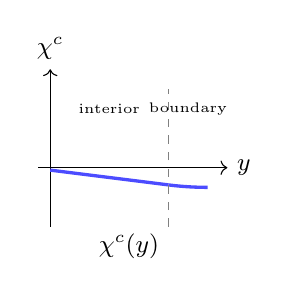
\begin{tikzpicture}[scale=0.5]
    \draw[->] (-0.3,0) -- (4.5,0) node[right] {\small $y$};
    \draw[->] (0,-1.5) -- (0,2.5) node[above] {\small $\chi^c$};

    % chi^c piecewise
    % interior: y in [0, 0.75), chi^c(y) = -0.0625 - 0.5y
    \draw[blue!70, very thick, domain=0:0.75] plot (\x*4, {-0.0625 - 0.5*\x});
    % boundary at x=1: y in [0.75, 1], chi^c(y) = (1-y)^2 - 0.5
    \draw[blue!70, very thick, domain=0.75:1] plot (\x*4, {(1-\x)*(1-\x) - 0.5});

    % Mark regions
    \draw[gray, dashed] (3, -1.5) -- (3, 2);
    \node[font=\tiny] at (1.5, 1.5) {interior};
    \node[font=\tiny] at (3.5, 1.5) {boundary};

    \node at (2, -2) {\small $\chi^c(y)$};
\end{tikzpicture}

\vspace{0.3cm}
\textbf{(c), (d)} In general:
\[
\chi^{c\bar{c}} \neq \chi
\]
but $\chi^{c\bar{c}} \geq \chi$ always!

$\chi^{c\bar{c}} = \chi$ iff $\chi$ is c-concave.
\end{center}
\end{column}
\end{columns}
\end{frame}

%==============================================================================
\section{Existence of Dual Optimizers}
%==============================================================================

\begin{frame}{Improving Dual Pairs via c-Transform}
\textbf{Key observation:} Given any admissible pair $(\phi, \psi)$ for (DP), we can \textbf{improve} it:

\vspace{0.3cm}
\textbf{Step 1:} Replace $\psi$ with $\phi^c$:
\begin{itemize}
    \item $\phi^c(y) = \inf_x [c(x,y) - \phi(x)]$
    \item Check: $\phi(x) + \phi^c(y) \leq c(x,y)$ automatically! \checkmark
    \item Since $\psi \leq \phi^c$ (from original constraint), we have $\int \phi^c \, d\nu \geq \int \psi \, d\nu$
\end{itemize}

\vspace{0.3cm}
\textbf{Step 2:} Replace $\phi$ with $(\phi^c)^{\bar{c}} = \phi^{c\bar{c}}$:
\begin{itemize}
    \item Same argument shows improvement
\end{itemize}

\vspace{0.3cm}
\textbf{Result:} Can always assume optimal $(\phi^*, \psi^*)$ satisfies:
\[
\psi^* = (\phi^*)^c \quad \text{and} \quad \phi^* \text{ is c-concave}
\]
\end{frame}

%==============================================================================
\begin{frame}{Proposition 1.11: Existence of Dual Solution}
\begin{block}{Proposition 1.11}
Suppose $X$ and $Y$ are \textbf{compact} and $c$ is \textbf{continuous}. Then:
\begin{enumerate}
    \item There exists a solution $(\phi, \psi)$ to (DP)
    \item It has the form: $\phi \in c\text{-conc}(X)$, $\psi = \phi^c$
\end{enumerate}
\vspace{-0.2cm}
\[
\max(\text{DP}) = \max_{\phi \in c\text{-conc}(X)} \left[ \int_X \phi \, d\mu + \int_Y \phi^c \, d\nu \right]
\]
\vspace{-0.3cm}
\end{block}

\textbf{Proof sketch:}
\begin{enumerate}
    \setlength{\itemsep}{0pt}
    \item Take maximizing sequence, improve to c-concave form
    \item c-concave functions are equicontinuous
    \item Normalize: $\min \phi_n = 0$
    \item Equibounded: $\phi_n, \psi_n$ bounded
    \item Ascoli-Arzel\`a $\Rightarrow$ convergent subsequence
    \item Limit is admissible and optimal \hfill $\square$
\end{enumerate}
\end{frame}

%==============================================================================
\begin{frame}{Visualization: Optimizing in c-concave Class}
\begin{center}
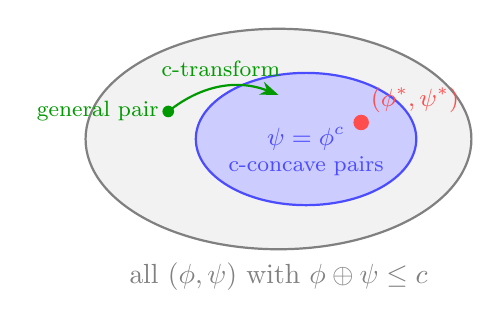
\begin{tikzpicture}[scale=0.7]
    % All dual feasible
    \draw[gray, thick, fill=gray!10] (0,0) ellipse (3.5 and 2);
    \node[gray] at (0, -2.5) {all $(\phi,\psi)$ with $\phi \oplus \psi \leq c$};

    % c-concave subset
    \draw[blue!70, thick, fill=blue!20] (0.5,0) ellipse (2 and 1.2);
    \node[blue!70, font=\small] at (0.5, 0) {$\psi = \phi^c$};
    \node[blue!70, font=\footnotesize] at (0.5, -0.5) {c-concave pairs};

    % Optimal point
    \fill[red!70] (1.5, 0.3) circle (4pt);
    \node[red!70, above right, font=\small] at (1.5, 0.3) {$(\phi^*, \psi^*)$};

    % Arrow showing improvement
    \draw[-{Stealth}, green!60!black, thick] (-2, 0.5) to[bend left] node[above, font=\footnotesize] {c-transform} (0, 0.8);
    \fill[green!60!black] (-2, 0.5) circle (3pt);
    \node[green!60!black, left, font=\footnotesize] at (-2, 0.5) {general pair};
\end{tikzpicture}
\end{center}

\vspace{0.3cm}
\textbf{Key insight:} Optimizing over c-concave pairs is sufficient, and this set has good compactness properties!
\end{frame}

%==============================================================================
\section{Kantorovich Potentials}
%==============================================================================

\begin{frame}{Definition 1.12: Kantorovich Potentials}
\begin{block}{Definition}
A function $\phi$ realizing the maximum in (DP) is called a \textbf{Kantorovich potential} for the transport from $\mu$ to $\nu$.
\end{block}

\vspace{0.3cm}
\textbf{Properties:}
\begin{itemize}
    \item Can always choose $\phi$ to be c-concave
    \item $\psi = \phi^c$ is the corresponding ``conjugate'' potential
    \item Kantorovich potentials may not be unique (can add constants)
\end{itemize}

\vspace{0.4cm}
\textbf{Duality formula:}
\[
\boxed{\min(\text{KP}) = \max_{\phi \in c\text{-conc}(X)} \left[ \int_X \phi \, d\mu + \int_Y \phi^c \, d\nu \right]}
\]

\vspace{0.2cm}
\textbf{Implication:} $\min(\text{KP})$ is a \textbf{convex function} of $(\mu, \nu)$ (supremum of linear functionals).
\end{frame}

%==============================================================================
\begin{frame}{Optimality Conditions}
\textbf{Complementary slackness:} If $\gamma^*$ is optimal for (KP) and $(\phi^*, \psi^*)$ is optimal for (DP):

\vspace{0.3cm}
\[
\boxed{\phi^*(x) + \psi^*(y) = c(x,y) \quad \gamma^*\text{-almost everywhere}}
\]

\vspace{0.3cm}
\textbf{Equivalently:} $\gamma^*$ is concentrated on the set
\[
\Gamma := \{(x,y) : \phi^*(x) + \psi^*(y) = c(x,y)\}
\]

\vspace{0.4cm}
\begin{center}
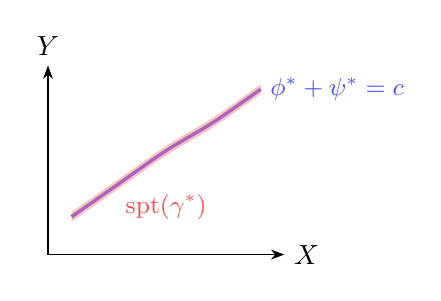
\begin{tikzpicture}[scale=0.6]
    \draw[-{Stealth}] (0,0) -- (5,0) node[right] {$X$};
    \draw[-{Stealth}] (0,0) -- (0,4) node[above] {$Y$};

    % Cost surface and equality set
    \draw[blue!70, very thick] plot[smooth] coordinates {(0.5,0.8) (1.5,1.5) (2.5,2.2) (3.5,2.8) (4.5,3.5)};
    \node[blue!70, right] at (4.5, 3.5) {\small $\phi^* + \psi^* = c$};

    % Gamma support
    \fill[red!50, opacity=0.5] plot[smooth] coordinates {(0.5,0.7) (1.5,1.4) (2.5,2.1) (3.5,2.7) (4.5,3.4)}
        -- plot[smooth] coordinates {(4.5,3.6) (3.5,2.9) (2.5,2.3) (1.5,1.6) (0.5,0.9)} -- cycle;

    \node[red!70] at (2.5, 1) {\small $\text{spt}(\gamma^*)$};
\end{tikzpicture}
\end{center}
\end{frame}

%==============================================================================
\begin{frame}{Exercise 3: Finding Kantorovich Potentials}
\textbf{Problem:} Let $X = Y = [0,1]$, $c(x,y) = |x-y|$, and
\[
\mu = \Ld|_{[0,1]}, \quad \nu = \Ld|_{[0,1]}
\]
(both uniform on $[0,1]$).

\vspace{0.3cm}
\textbf{Questions:}
\begin{enumerate}
    \item[(a)] What is the optimal transport map $T$?
    \item[(b)] What is the optimal transport cost?
    \item[(c)] Find Kantorovich potentials $(\phi, \psi)$ such that $\phi(x) + \psi(y) \leq |x-y|$ and equality holds on $\{(x, T(x))\}$.
    \item[(d)] Verify strong duality.
\end{enumerate}

\vspace{0.3cm}
\textit{Hint:} When $\mu = \nu$, the optimal transport is often ``stay in place.''
\end{frame}

%==============================================================================
\begin{frame}{Solution 3}
\begin{columns}
\begin{column}{0.55\textwidth}
\textbf{(a)} Optimal map: $T(x) = x$ (identity)

Since $\mu = \nu$, staying in place costs nothing.

\vspace{0.2cm}
\textbf{(b)} Optimal cost:
\[
\int_0^1 |x - T(x)| \, dx = \int_0^1 0 \, dx = 0
\]

\vspace{0.2cm}
\textbf{(c)} Need $\phi(x) + \psi(y) \leq |x-y|$ with equality at $y = x$.

At $y = x$: $\phi(x) + \psi(x) = 0$

Choose: $\phi(x) = 0$, $\psi(y) = 0$

Check: $0 + 0 = 0 \leq |x-y|$ for all $x,y$ \checkmark

\vspace{0.2cm}
\textbf{(d)} $\int \phi \, d\mu + \int \psi \, d\nu = 0 + 0 = 0$

Strong duality: $0 = 0$ \checkmark
\end{column}
\begin{column}{0.45\textwidth}
\begin{center}
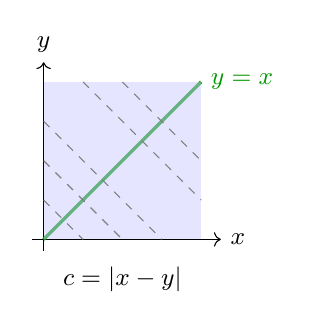
\begin{tikzpicture}[scale=0.5]
    \draw[->] (-0.3,0) -- (4.5,0) node[right] {\small $x$};
    \draw[->] (0,-0.3) -- (0,4.5) node[above] {\small $y$};

    % Diagonal (T = id)
    \draw[green!60!black, very thick] (0,0) -- (4,4);
    \node[green!60!black, right] at (4, 4) {\small $y = x$};

    % Cost constraint region
    \fill[blue!20, opacity=0.5] (0,0) -- (4,0) -- (4,4) -- (0,4) -- cycle;

    % Level sets of |x-y|
    \draw[gray, dashed] (0,1) -- (1,0);
    \draw[gray, dashed] (0,2) -- (2,0);
    \draw[gray, dashed] (0,3) -- (3,0);
    \draw[gray, dashed] (1,4) -- (4,1);
    \draw[gray, dashed] (2,4) -- (4,2);

    \node at (2, -1) {\small $c = |x-y|$};
\end{tikzpicture}

\vspace{0.3cm}
\textbf{Note:} $\phi = \psi = 0$ is one choice.

Other valid: $\phi = k$, $\psi = -k$ for any $k \leq 0$.
\end{center}
\end{column}
\end{columns}
\end{frame}

%==============================================================================
\section{Summary}
%==============================================================================

\begin{frame}{Summary: Duality in Optimal Transport}
\textbf{Primal Problem (KP):}
\[
\min_{\gamma \in \Pi(\mu,\nu)} \int_{X \times Y} c \, d\gamma
\]

\vspace{0.2cm}
\textbf{Dual Problem (DP):}
\[
\max_{\phi \oplus \psi \leq c} \left[ \int_X \phi \, d\mu + \int_Y \psi \, d\nu \right]
\]

\vspace{0.3cm}
\textbf{Key Results:}
\begin{itemize}
    \item \textbf{Weak Duality:} $\sup(\text{DP}) \leq \min(\text{KP})$ (always)
    \item \textbf{Strong Duality:} $\max(\text{DP}) = \min(\text{KP})$ (under mild conditions)
    \item \textbf{Existence:} Optimal dual pair exists when $X, Y$ compact, $c$ continuous
    \item \textbf{c-Transform:} Can restrict to c-concave potentials $\phi$, $\psi = \phi^c$
    \item \textbf{Complementary Slackness:} $\phi^* + \psi^* = c$ on $\text{spt}(\gamma^*)$
\end{itemize}

\vspace{0.2cm}
\textbf{Key Tools:} Ascoli-Arzel\`a, c-transform, continuity of inf/sup
\end{frame}

%==============================================================================
\begin{frame}{Looking Ahead}
\textbf{Next topics:}

\vspace{0.3cm}
\begin{itemize}
    \item \textbf{Section 1.3:} Strictly convex costs $c(x,y) = h(x-y)$
    \begin{itemize}
        \item Existence of optimal transport \textbf{maps}
        \item Brenier's theorem for quadratic cost
    \end{itemize}

    \vspace{0.3cm}
    \item \textbf{Section 1.6:} c-concavity and optimality
    \begin{itemize}
        \item c-cyclical monotonicity
        \item Direct proof of strong duality
        \item Sufficient conditions for optimality
    \end{itemize}
\end{itemize}

\vspace{0.4cm}
\textbf{Key question:} When does the optimal \textbf{plan} come from a \textbf{map}?
\[
\gamma^* = (\text{id}, T)_\# \mu \quad \text{for some } T: X \to Y
\]
\end{frame}

\end{document}
